% =====================================================================
\chapter{Functional architecture}
% =====================================================================
The architecture is described in two parts. The \emph{online} part is the
service that handles requests from patients, doctors and the manager. The
\emph{offline} part concerns the training of the prediction model, which
supports the online service and is separate from the normal handling of
requests.

\section{Online architecture}
Figure~\ref{fig:architecture} shows the functional components of the online
service. The three actors reach the system through a single access control
component, which sends each request only to the service the role is entitled
to: the patient to their own data, the doctor to the assigned patients, and
the manager to aggregated data only. The services read and write a common data
archive. The CGM sensor writes the glucose samples directly into the archive,
in a flow that is separate from the prediction requests. The prediction service
uses the model made available by the offline training process.

\begin{figure}[H]
    \centering
    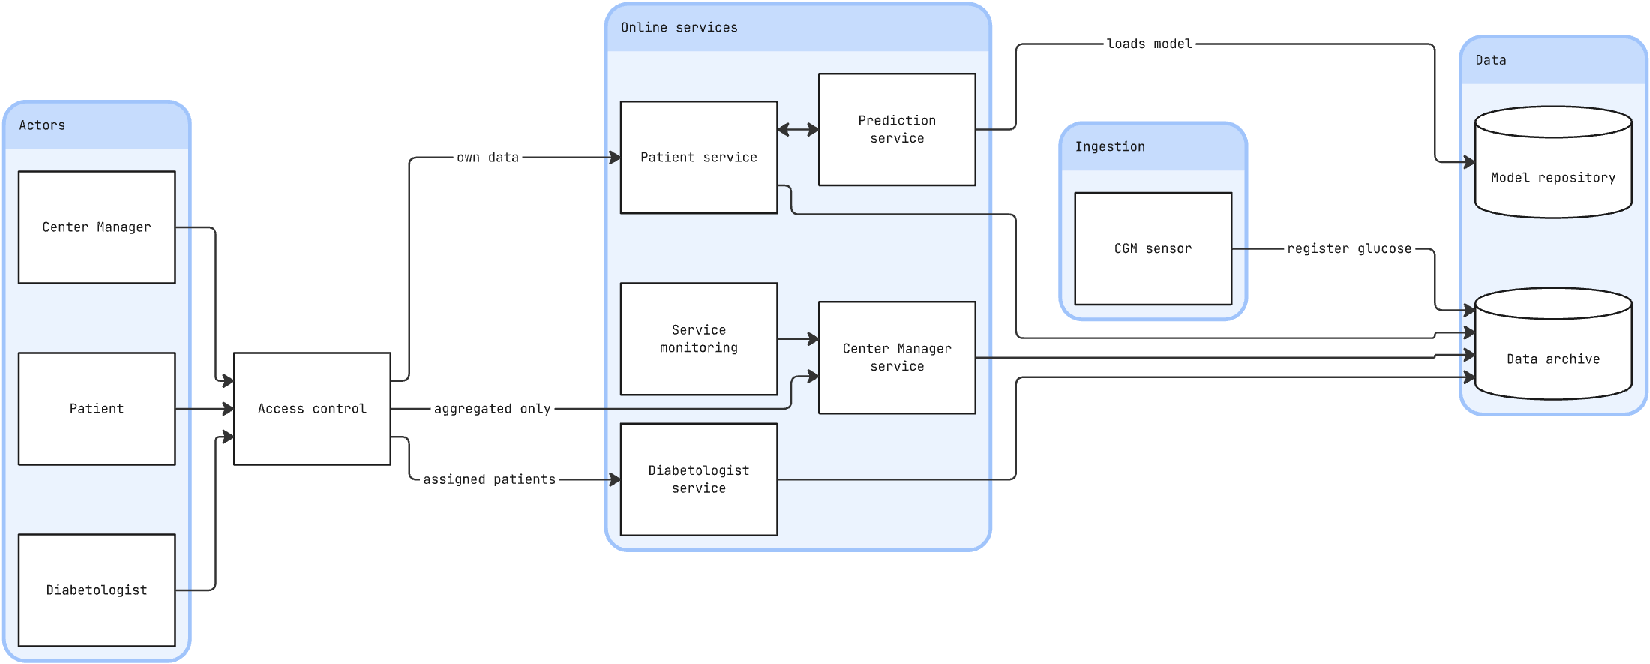
\includegraphics[width=1\linewidth]{attach/architecture.pdf}
    \caption{Functional architecture of the online service.}
    \label{fig:architecture}
\end{figure}


\section{Offline model training}
\label{sec:offline}
The system includes an offline process for training the prediction model
using historical patient data. The resulting model is made available to
the online service, which uses it to generate glucose predictions.
The training process is separate from the normal operation of the
online service and does not interfere with patient requests (RF19, RNF10).

The prediction engine relies on a unified global model trained on multicentric
patient cohorts (OhioT1DM dataset). Rather than maintaining thousands of isolated
per-patient models—which would introduce cold-start latency and severe memory overhead
in the cloud cluster—the model dynamically adapts to each individual's metabolic state
through their real-time autoregressive history (the preceding 60 minutes of glucose readings
and derivative trends). This design guarantees immediate availability for newly registered
patients while keeping cloud serving lightweight and horizontally scalable (RF20).

\section{Components}
Table~\ref{tab:components} describes each component of
Figure~\ref{fig:architecture}: what it does and which requirements it
satisfies.

\begingroup
\small
\setlength{\LTpre}{4pt}\setlength{\LTpost}{6pt}
\begin{longtable}{>{\bfseries\raggedright\arraybackslash}p{2.9cm}>{\raggedright\arraybackslash}p{\dimexpr\linewidth-5.6cm-6\tabcolsep\relax}>{\raggedright\arraybackslash}p{2.7cm}}\caption{Components of the online architecture, their responsibilities and requirements.}
\label{tab:components}\\
\toprule
\rowcolor{accent}\tablehead{Component} & \tablehead{What it does} & \tablehead{Requirements}\\
\midrule\endfirsthead
\toprule
\rowcolor{accent}\tablehead{Component} & \tablehead{What it does} & \tablehead{Requirements}\\
\midrule\endhead
\bottomrule\endfoot
Access control & Authenticates every user, assigns the role and forwards each request only to the service the role is entitled to. The control is made on the server and applies to the data, not only to the screens. & RF01, RF02, RNF08, RNF09\\
\rowcolor{softgrey}
Patient service & Receives the carbohydrates declared for a meal, reads the recent history of the patient, asks the prediction service for the 30-minute forecast, returns the outcome message, records a flag for the doctor when hyperglycemia or hypoglycemia is predicted, and gives the patient access to their own history. & RF03, RF05--RF08, RNF01, RNF07\\
Prediction service & Loads the unified prediction model from the model repository and computes the 30-minute glucose forecast and risk classification from recent CGM measurements and meal inputs. Serves all patients immediately without per-patient retraining. & RF05, RF20, RNF01, RNF02\\
\rowcolor{softgrey}
Diabetologist service & Shows the doctor the table of the assigned patients with their flags, the trend of each patient, the comparison between predicted and measured glucose with the deviations, and the detected trends. Allows registering new patients, setting and updating the diet, and recording interventions. & RF09--RF15, RF21, RNF08\\
Center Manager service & Builds the aggregated statistics shown in the dashboard, such as the interventions by cause, the accuracy of the predictions and the average regularity of the patients, without exposing the data of single patients. & RF16, RF17, RF18, RNF09\\
\rowcolor{softgrey}
Service monitoring & Collects response times, availability and compliance with the service level agreement, and passes them to the Center Manager service. & RF18, RNF01, RNF05, RNF06\\
CGM sensor & In this project it is simulated by replaying time series from the OhioT1DM dataset. Produces one glucose sample every five minutes for each monitored patient and registers it in the data archive. & RF04, RNF04\\
\rowcolor{softgrey}
Data archive & Stores meals and carbohydrates, measured glucose, predictions and deviations, flags, diets, assignments of patients to doctors and interventions. & RF03--RF18, RNF04\\
Model repository & Holds the validated versions and cryptographic checksums of the prediction model produced by offline training. New versions can be deployed via rolling updates without service interruption. & RF19, RNF10\\
\end{longtable}
\endgroup

\section{Access control}
Each actor accesses only the data and the functions of their competence.
The rule applies both to the data and to the views of the application. The check is made by the server (RNF08), and the health data are
protected in transit and at rest (RNF09).

\begin{figure}[H]
    \centering
    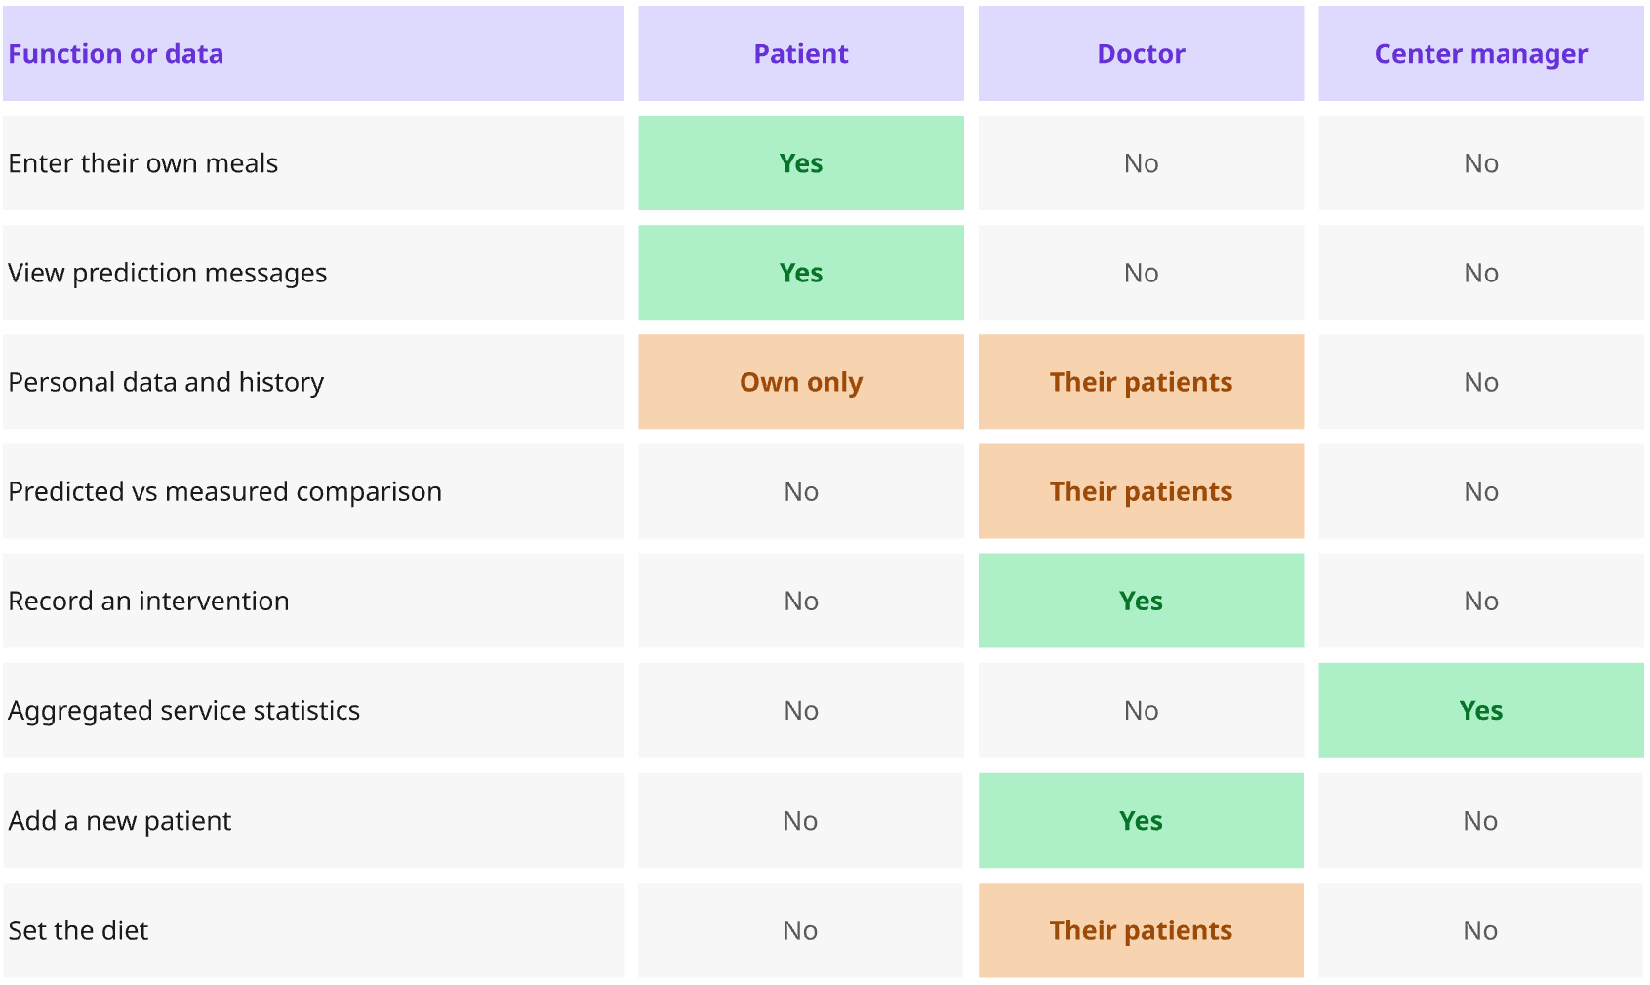
\includegraphics[width=\linewidth]{attach/permissions_table.pdf}
    \caption{Permissions of each actor.}
    \label{fig:permissions}
\end{figure}

% =====================================================================
\section{System behavior}
% =====================================================================
This section shows how the components interact in the main use cases through
sequence diagrams. In every diagram the access component first checks the
identity and the role of the user (UC01). 

\subsection{The patient declares a meal (UC02)}
Figure~\ref{fig:seq-meal} shows the core of the application. The patient logs
in and enters the carbohydrates of the meal. The patient service reads the
recent history of the patient from the data archive, passes a window of data
and the declared carbohydrates to the model, and receives the glucose predicted
at thirty minutes. The meal and the prediction are saved, and the outcome
depends on the prediction:
\begin{itemize}
  \item if the prediction is within the limits, the patient may proceed, with a
  warning if the carbohydrates exceed the diet;
  \item if hyperglycemia is predicted, the patient is told that the amount is
  excessive and a flag for the doctor is recorded;
  \item if hypoglycemia is predicted, the patient is told that the amount is
  insufficient and a flag for the doctor is recorded.
\end{itemize}
The doctor does not receive an instant notification and sees the flag during the
periodic review.

Under the hood, the prediction engine classifies the projected glucose into the seven clinical risk bands standard in diabetology (OhioT1DM benchmark). The system maps these granular clinical tiers into the four patient-facing macro-outcomes: target levels correspond to \emph{regular}; borderline levels trigger a \emph{warning}; and values below 3.9\,mmol/L (70\,mg/dL) or above 10.0\,mmol/L (180\,mg/dL) trigger the respective \emph{hypoglycemia} or \emph{hyperglycemia} risk flags.

\begin{figure}[H]
\centering
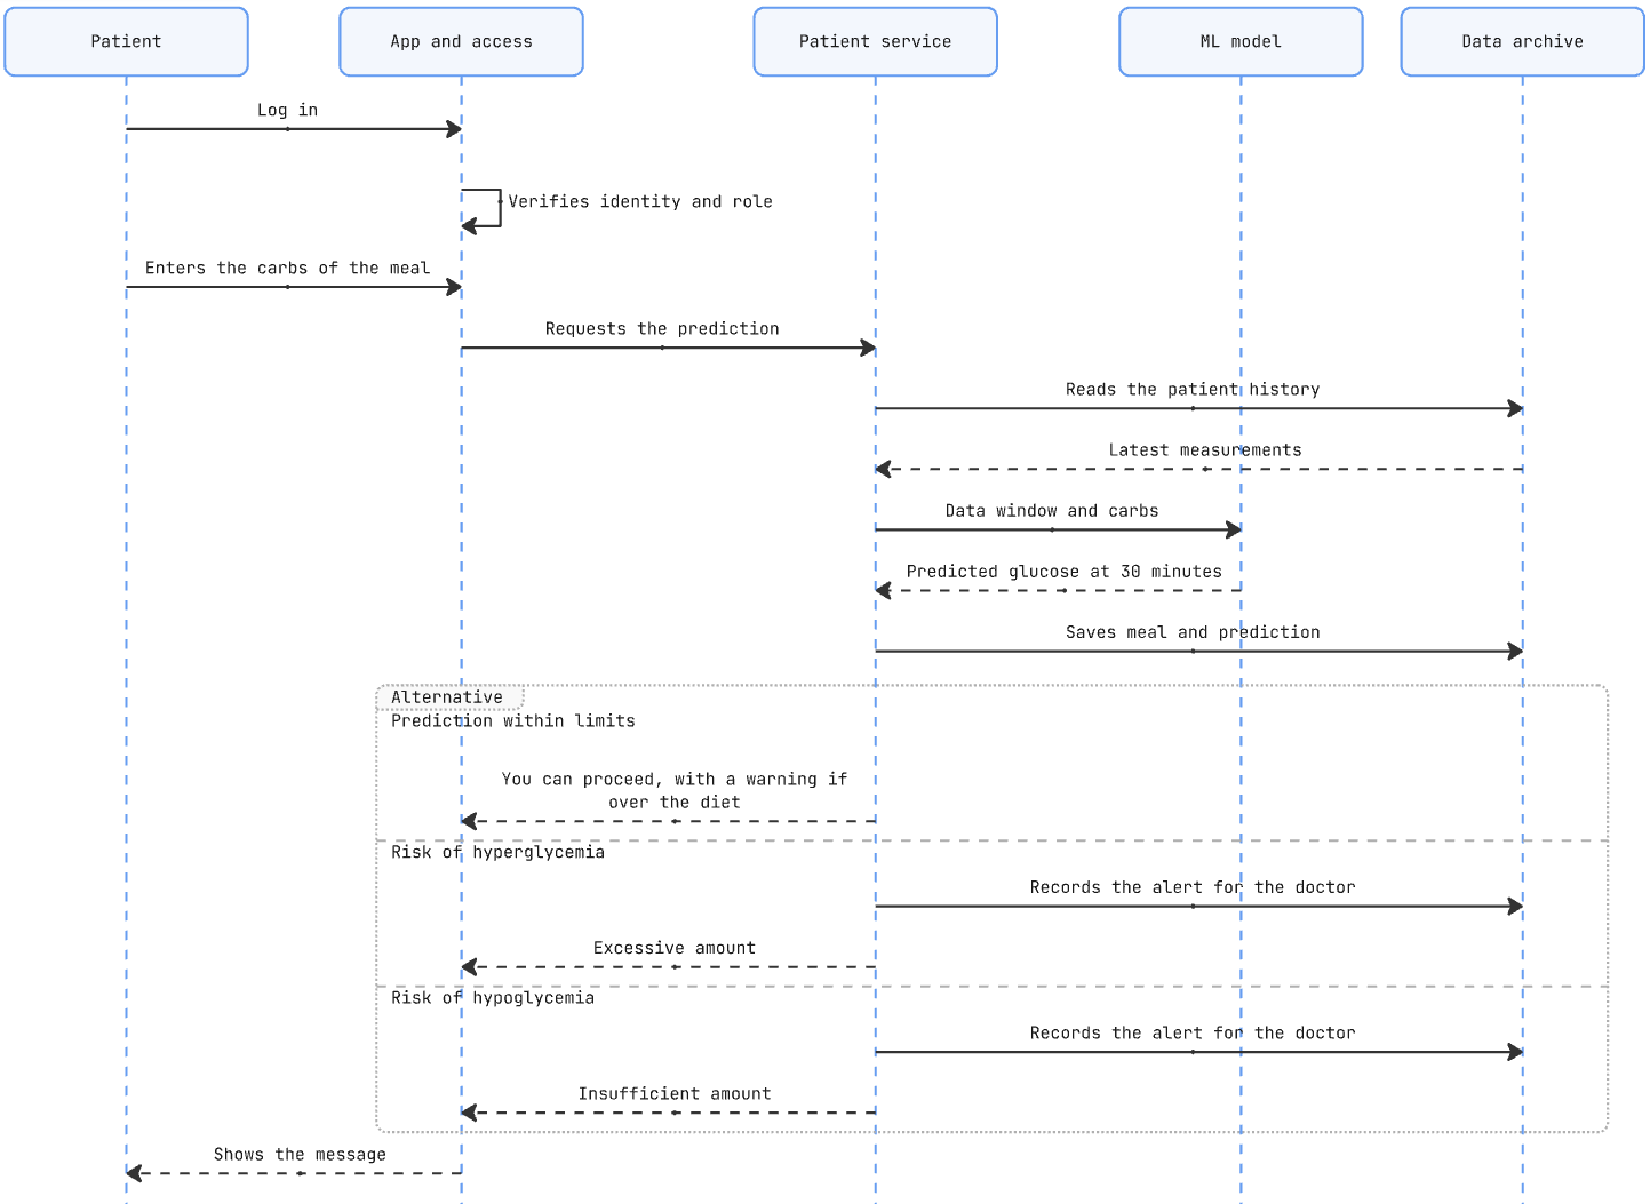
\includegraphics[width=\linewidth,height=0.76\textheight,keepaspectratio]{attach/seq_patient_meal.pdf}
\caption{Sequence diagram: the patient declares a meal and receives the outcome.}
\label{fig:seq-meal}
\end{figure}

\subsection{The doctor reviews the patients (UC04, UC05, UC06)}
In the periodic review (Figure~\ref{fig:seq-review}) the doctor opens a table
with only the patients assigned to them, with the flags received. After
selecting a patient, the doctor sees the trend over time, with the predicted
values compared with the measured ones. Before reading the data, the doctor
service checks that the patient is really assigned to that doctor. If an
intervention is needed, such as a reminder or a change of the diet, the doctor
records it and indicates whether the cause is a model error or the behavior of
the patient.

\begin{figure}[H]
\centering
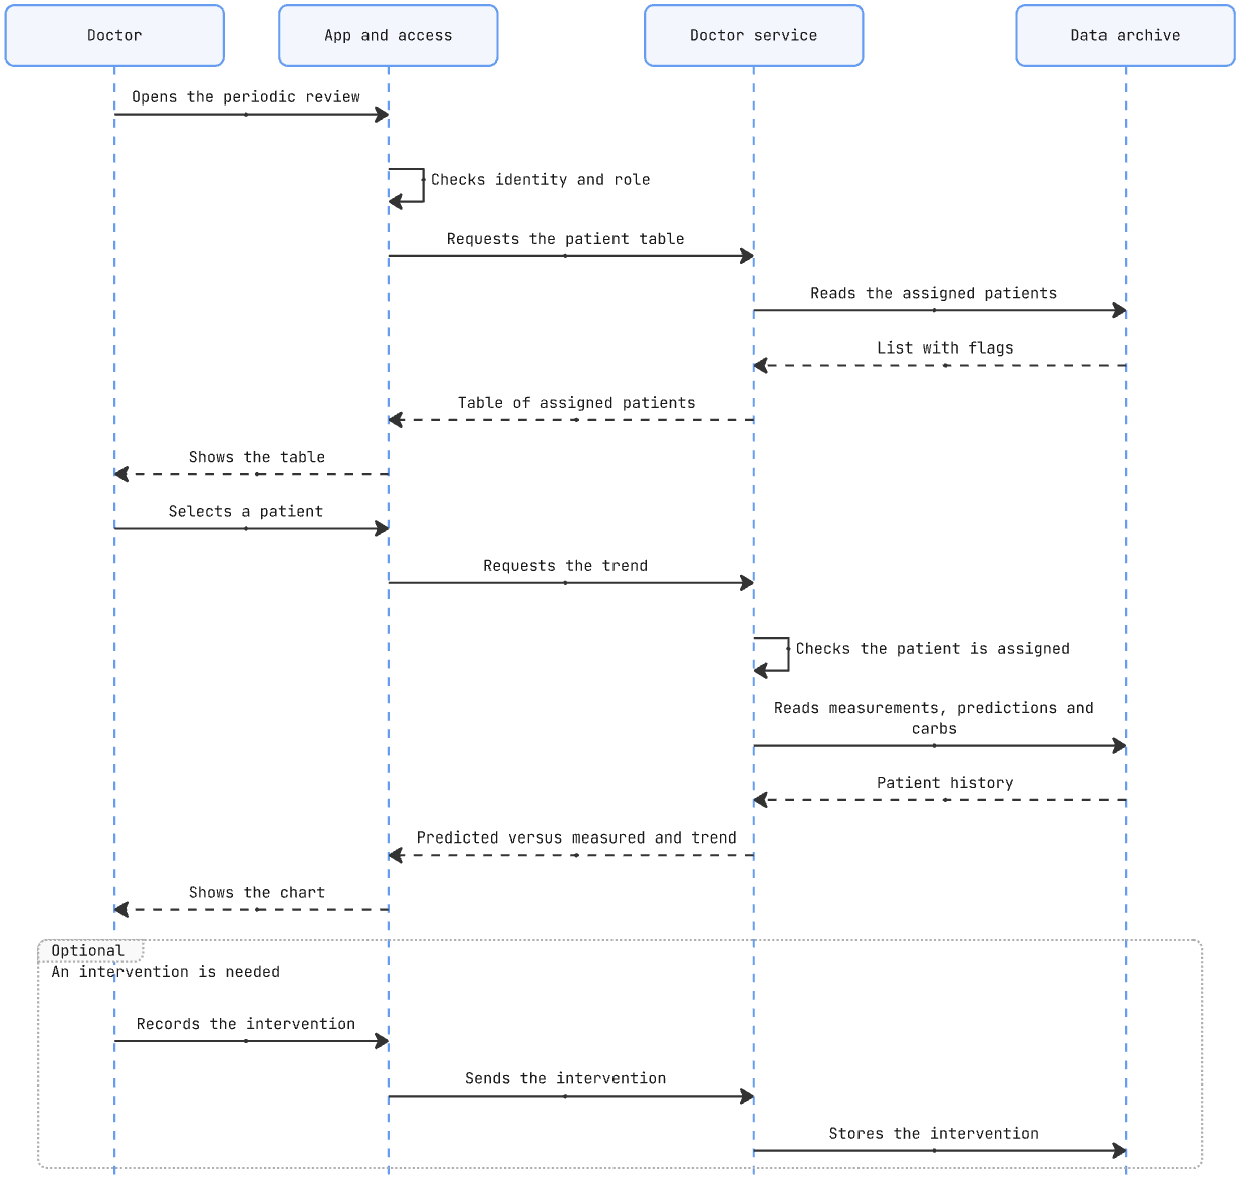
\includegraphics[width=\linewidth]{attach/seq_doctor_review.pdf}
\caption{Sequence diagram: the doctor reviews the assigned patients.}
\label{fig:seq-review}
\end{figure}

\subsection{The doctor registers a new patient (UC07)}
Figure~\ref{fig:seq-newpatient} shows how a new patient enters the system. The
doctor registers the patient, assigns them to their care, and sets the initial
diet. Thanks to the pre-trained unified global model, no per-patient retraining is
required; as soon as the initial 60-minute window of CGM readings is acquired,
the patient is immediately ready to receive predictions.

\begin{figure}[H]
\centering
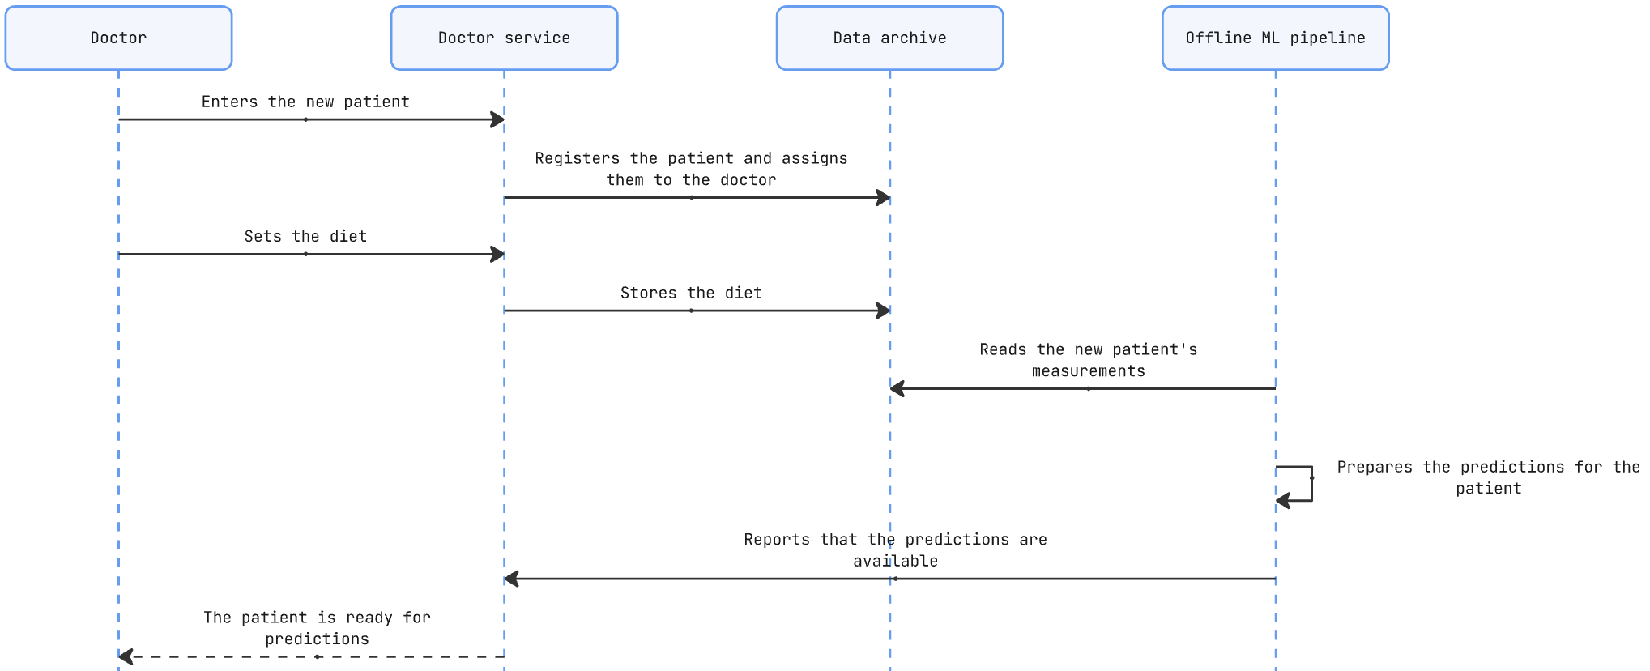
\includegraphics[width=\linewidth,height=0.72\textheight,keepaspectratio]{attach/seq_new_patient.pdf}
\caption{Sequence diagram: the doctor registers a new patient.}
\label{fig:seq-newpatient}
\end{figure}

\subsection{The center manager views the dashboard (UC08)}
The manager (Figure~\ref{fig:seq-dashboard}) opens the dashboard of the service
after logging in. The manager service reads counts and aggregated metrics from
the data archive: interventions by cause, accuracy of the predictions, average
regularity of the patients, response times and availability. It aggregates them
by period and by patient behavior, and returns aggregated statistics only. No
clinical data of single patients reaches the manager.

\begin{figure}[H]
\centering
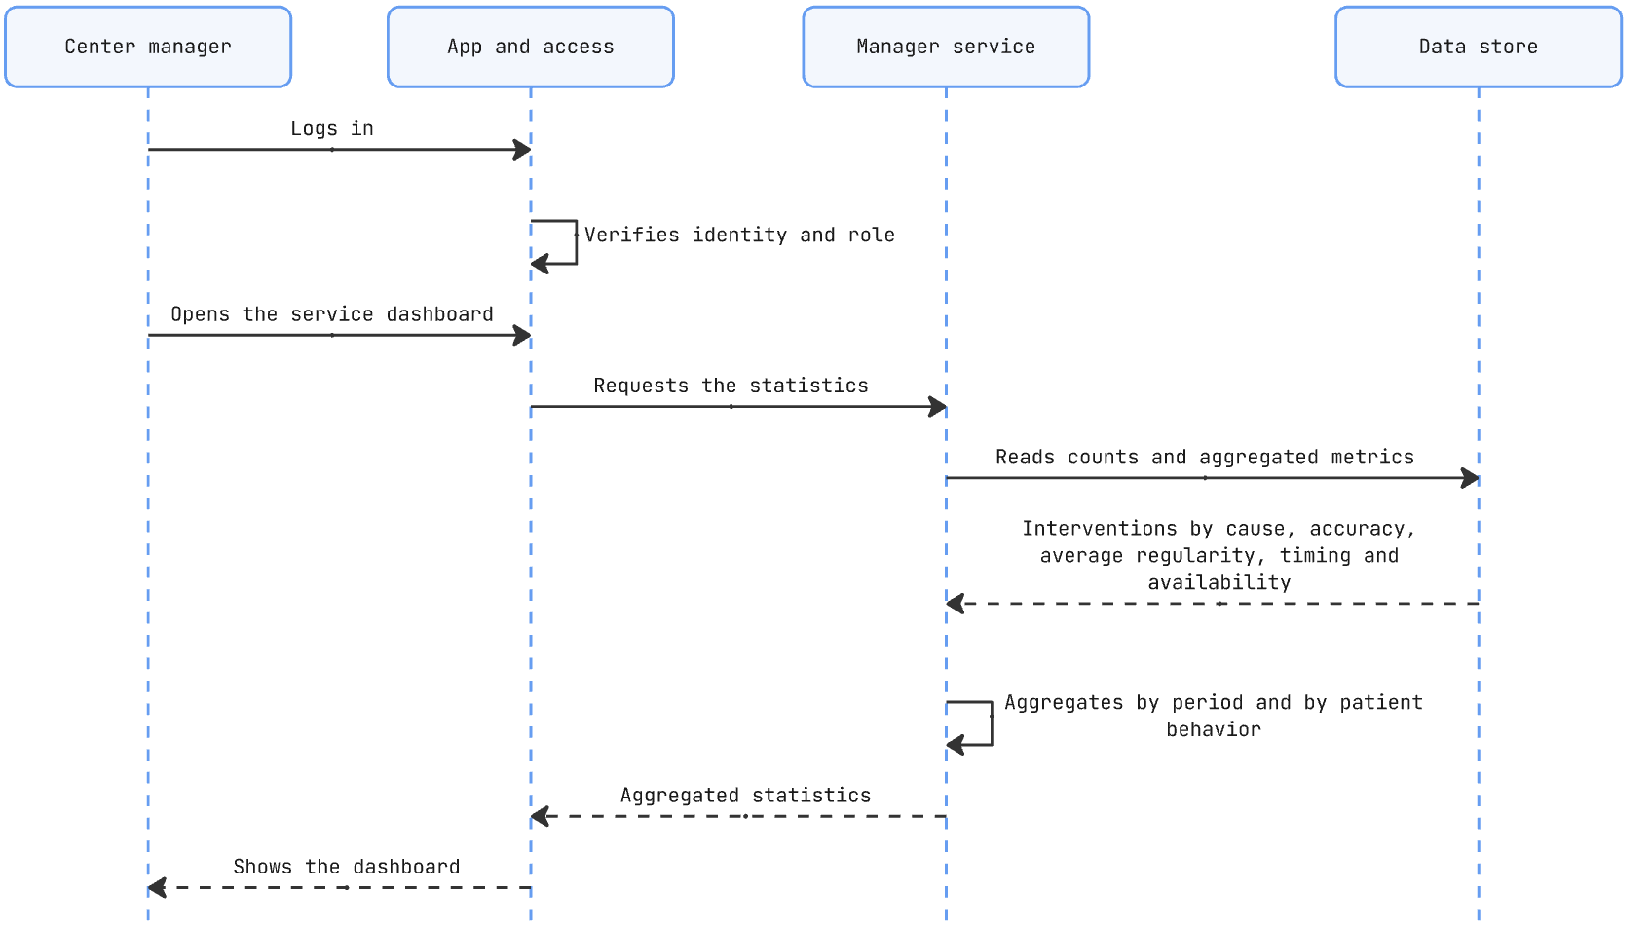
\includegraphics[width=\linewidth,height=0.72\textheight,keepaspectratio]{attach/seq_manager_dashboard.pdf}
\caption{Sequence diagram: the center manager views the service dashboard.}
\label{fig:seq-dashboard}
\end{figure}

\section{Mockups}
\label{sec:mockups}

To give an idea of what each actor sees, Figure~\ref{fig:mockups} shows
three early sketches of the main screens: the patient app, the doctor
dashboard and the center manager dashboard. They may differ in the final version of the application, which will have both mobile and desktop views.


\begin{figure}[htbp]
  \centering
  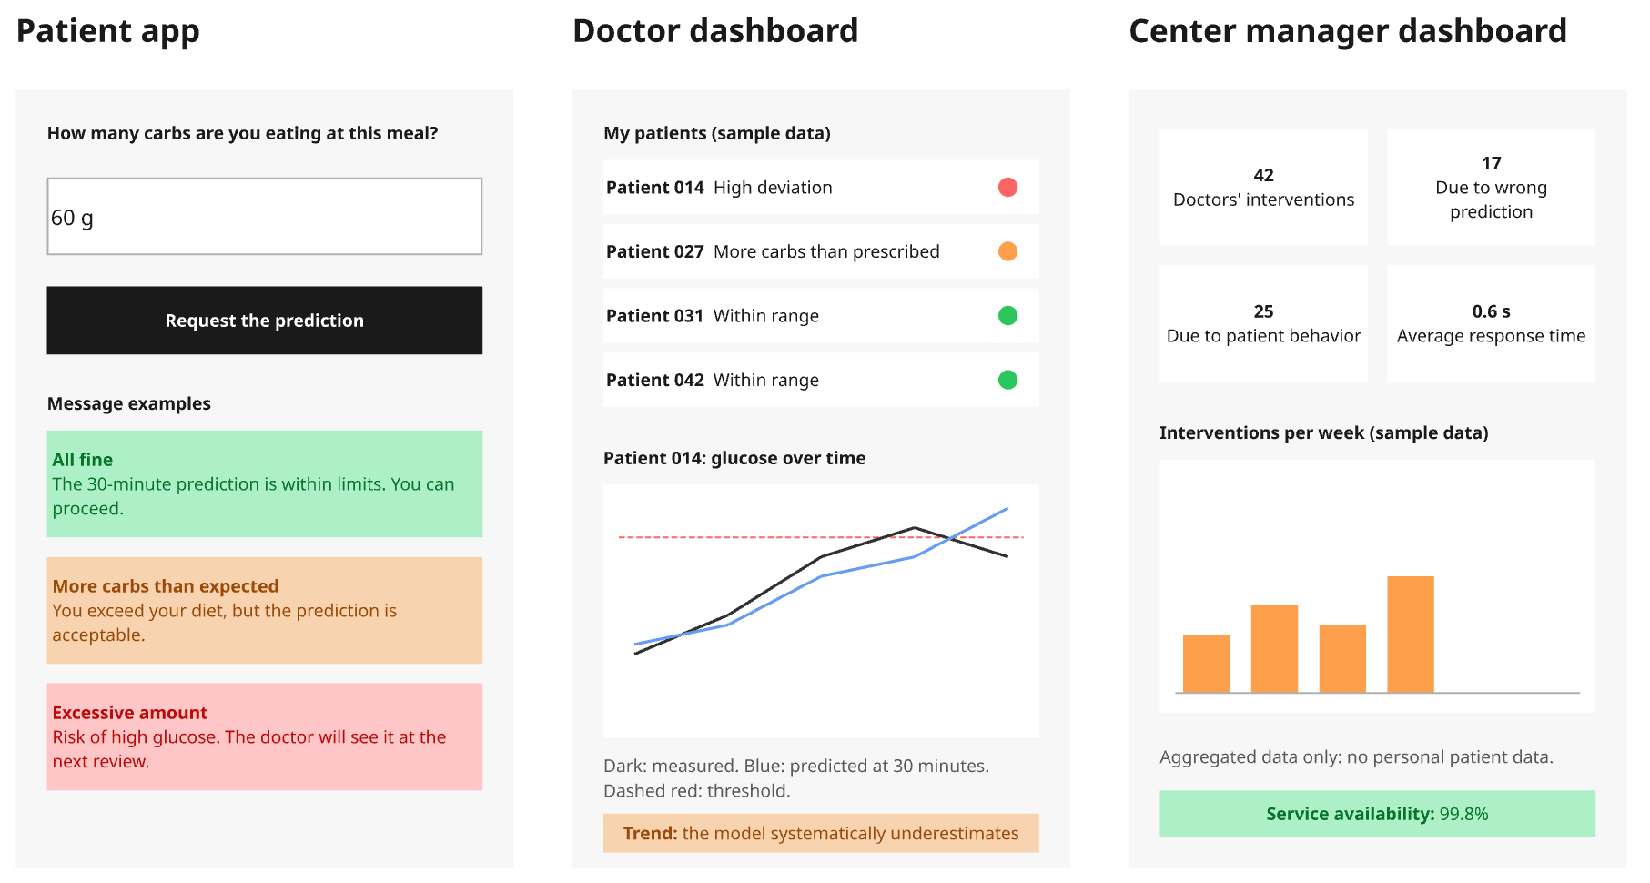
\includegraphics[width=\textwidth]{attach/mockup.pdf}
  \caption{Early mockups of the patient app, the doctor dashboard and the
  center manager dashboard (sample data).}
  \label{fig:mockups}
\end{figure}



